\subsection{Our Improved Approach (IHub)}

\subsubsection{Avoiding node pairs with no common neighbors}

As noted earlier, there are a vast number of node pairs $(a, c)$ in a graph with no common neighbors, i.e., $\Gamma_a \cap \Gamma_c = \phi$ (here $\Gamma_a$ represents the neighbors of vertex $a$), and thus have a similarity score of $0$. This is especially true for large sparse graphs. To address this, we limit computation of similarity scores of each vertex $a$ in the graph to its second order neighbors $c$, i.e., to vertices that are neighbors of the immediate neighbors $a$. We do this with a Depth First Search (DFS) traversal from each vertex $a$, limited to a distance of $2$.


\subsubsection{Finding common neighbors faster}

To expedite the identification of common neighbors between each vertex $a$ and its second-order neighbors $c$, we employ a hashtable. This hashtable keeps track of the frequency of visits to each second-order vertex $c$ during the DFS traversal, yielding the count of common neighbors $|\Gamma_a \cap \Gamma_c|$ in each hashtable entry (with $c$ as the key). This count reflects the number of paths from $a$ to $c$, as each common neighbor contributes a new path. For the JC metric, in addition to common neighbors, we need the total count of neighbors $\Gamma_a \cup \Gamma_c$ between $a$ and $c$. This count is easily calculated as $|\Gamma_a \cup \Gamma_c| = |\Gamma_a| + |\Gamma_c| - |\Gamma_a \cap \Gamma_c|$. To compute AA and RA similarity scores, we use a hashtable with floating-point values, and accumulate $1/\log{|\Gamma_b|}$ and $1/|\Gamma_b|$ respectively. Here, $b$ is a first-order neighbor of $a$ and a common neighbor between $a$ and $b$. Finally, to avoid redundancy in an undirected graph, we skip second-order neighbors $c$ where $c \leq a$. This also prevents the scoring (and prediction) of self-loops.


\subsubsection{Design of Hashtable}

As C++'s inbuilt \texttt{map} has poor performance, we employ collision-free per-thread hashtables (we discuss later about parallelization), similar to our previous work \cite{sahu2023gvelouvain}. An example of this hashtable for two threads is shown in Figure \ref{fig:about-hashtable}. Each hashtable includes a keys vector, a values vector (of size $|V|$), and a key count. The value associated with each key is stored or accumulated in the index pointed to by the key. To prevent false cache sharing, we independently update the key count of each hashtable and allocate it separately on the heap. As previously mentioned, the vertex IDs of second-order neighbors $c$ of each vertex $a$ serve as keys in the hashtable, and the associated values represent the number of times $c$ has been visited during a DFS traversal (of distance $2$) from $a$. For AA and RA scores, we use a hashtable with integral keys and floating-point values.

\begin{figure*}[hbtp]
  \centering
  \subfigure[Standard approach]{
    \label{fig:about-pruning--01}
    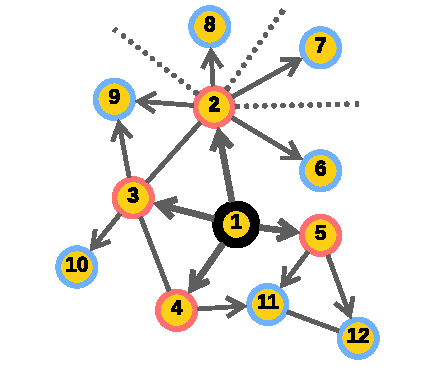
\includegraphics[width=0.31\linewidth]{out/about-pruning-01.pdf}
  }
  \subfigure[Disregard hubs with degree $> 8$]{
    \label{fig:about-pruning--02}
    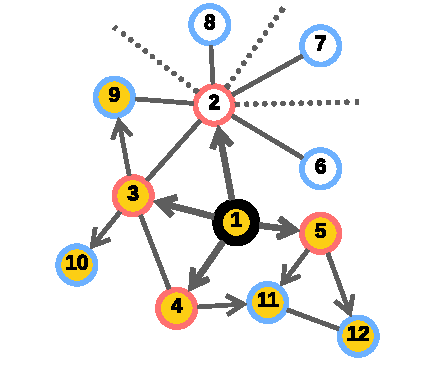
\includegraphics[width=0.31\linewidth]{out/about-pruning-02.pdf}
  }
  \subfigure[Disregard hubs with degree $> 4$]{
    \label{fig:about-pruning--03}
    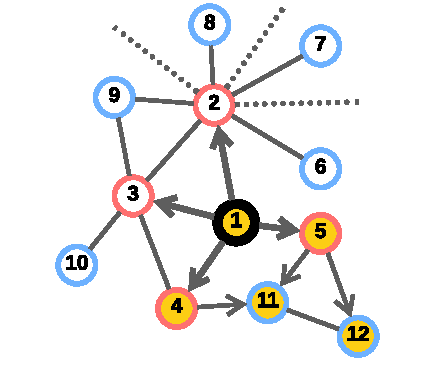
\includegraphics[width=0.31\linewidth]{out/about-pruning-03.pdf}
  } \\[-2ex]
  \caption{Illustration of our neighborhood-based link prediction approach, which disregards large hubs (first-order neighbors with high degree). The approach applies to each vertex in the graph. Here, we focus on the neighborhood of a vertex $1$ in the graph. The current vertex $1$ is outlined in black, its first-order neighbors in red, and its second-order neighbors in blue. Edge directions indicate traversal, with some second order vertices omitted for simplicity (dotted edges). (a) Depicts the standard approach, which considers all second-order neighbors of vertex $1$. (b) Presents our approach, which considers only second-order neighbors linked to $1$ through a small hub (degree $\leq 8$). This pruning reduces runtime and enhances prediction quality. (c) Illustrates our approach, where vertices with degree $> 4$ are considered large hubs.}
  \label{fig:about-pruning}
\end{figure*}

\begin{figure}[hbtp]
  \centering
  \subfigure{
    \label{fig:about-hashtable--all}
    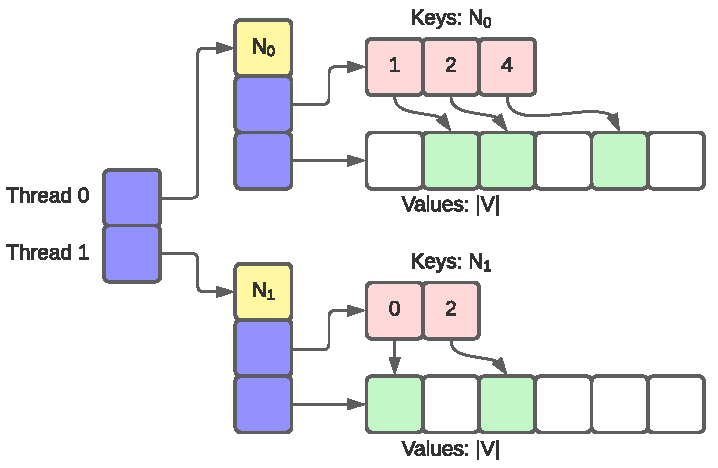
\includegraphics[width=0.88\linewidth]{out/about-hashtable.pdf}
  } \\[-2ex]
  \caption{Illustration of collision-free per-thread hashtables that are well separated in their memory addresses, for two threads. Each hashtable consists of a keys vector, a values vector (of size $|V|$), and a key count ($N_0$/$N_1$). The value associated with each key is stored/accumulated in the index pointed by the key. As the key count of each hashtable is updated independently, we allocate it separately on the heap to avoid false cache sharing \cite{sahu2023gvelouvain}. These are used in the scoring phase of our implementation to track common neighbors.}
  \label{fig:about-hashtable}
\end{figure}



\subsubsection{Avoiding first order neighbors}

Once the DFS traversal from vertex $a$ is complete, and all hashtable entries are populated, we clear the entries associated with the first-order neighbors $b$ of $a$. This precaution is necessary because some first-order neighbors of $a$ may have edges with the other first-order neighbors.


\subsubsection{Computing scores}

With all valid entries in the hashtable populated, we proceed to compute scores from vertex $a$ to each second-order neighbor $c$, using the appropriate formula for the selected metric as outlined in Section \ref{sec:metrics}. For CN, AA, and RA metrics, no additional computation is required, as the hashtable values already contain the desired scores.


\subsubsection{Tracking top-k edges}

Since storing all obtained similarity scores is impractical due to the scale of processed graphs, we use a min-heap based prediction list. This min-heap enables us to maintain the top-$k$ edges with the highest similarity scores per thread. It works by evicting the node pair with the lowest score when a new node pair with a higher score is encountered. As an optimization, we convert the per-thread prediction lists into a min-heap only after its have been populated with $k$ entries.


\subsubsection{Parallelizing the process}

To parallelize the computation, we partition the graph among threads, employing OpenMP's \textit{dynamic} schedule with a chunk size of $2048$ (to minimize work imbalance and scheduling overhead). Each partition is processed independently, with each thread using its own hashtable and prediction list. To account for the possibility of a single thread identifying all top-$k$ links globally, each thread employs a prediction list of size $k$. After individual thread predictions, we independently sort the per-thread top-$k$ predictions by score on each thread. These sorted lists are then merged into a global top-$k$ prediction list using a max-heap.

\ignore{An alternative approach to merge per-thread top-$k$ prediction lists involves concatenating the per-thread lists into a single prediction list, performing a parallel sort, and truncating all predicted edges except the top-$k$. However, this method can lead to out-of-memory crashes on large graphs due to the size of the concatenated prediction list.}

We call this approach IHub. It has a time complexity of $O(ND^2)$, where $N$ is the number of vertices in the graph, and $D$ is the maximum degree of a vertex in the graph.\ignore{It's worth noting that the results obtained by our parallel algorithm are non-deterministic. This is because multiple edges can have matching scores, and the order of edges with the same score may be random due to parallelism.}




\subsection{Our Heuristic Approach which Disregards Large Hubs (LHub)}

\subsubsection{Explanation of the approach}

To optimize link prediction further, we recognize that low-degree nodes, representing users with few connections in the social network, are more selective in accepting friend requests and are likely to form connections with people they have stronger, more meaningful relationships with, such as close friends and family. Thus, low-degree nodes confer significant similarity among their neighbors, while high-degree nodes generally do not (due to their lack of selectivity). We call such high-degree nodes as large hubs. Accordingly, for a given vertex $a$ and each of its immediate neighbors $b$, we only explore the neighbors $c \in \Gamma_b$ of $b$ if the degree of $b$ is within a certain threshold $L_H$, i.e., $|\Gamma_b| \leq L_H$. We call this threshold as the \textit{hub limit}. This minimizes DFS exploration of second-degree neighbors $c$ during computation of neighbor-based similarity scores.

We call this approach LHub. It has the same time complexity as IHub, i.e., $O(ND^2)$, but significantly outperforms it by runtime, while achieving the same or better prediction quality.


\subsubsection{A simple example}

Figure \ref{fig:about-pruning} demonstrates the LHub approach. Here, we consider the neighborhood of vertex $1$ in a graph, where $1$ is outlined in black, its first-order neighbors in red, its second-order neighbors in blue, and explored/traversed vertices are shown with a yellow fill. The arrows in the figure indicate the direction of DFS traversal, and for figure simplicity, three neighbors of vertex $2$ are omitted (shown with dotted edges).

\ignore{\paragraph{Standard approach (IHub)}}

Figure \ref{fig:about-pruning--01} depicts the standard approach, which considers all second-order neighbors of vertex $1$ for score computation, i.e. vertices $6$ to $12$. This is the process followed by the IHub approach.

\ignore{\paragraph{Disregards hubs with degree $> 8$ (LHub)}}

Figure \ref{fig:about-pruning--02} depicts our LHub approach. It considers only second-order neighbors linked to vertex $1$ by a small hub, with a degree $\leq 8$, for score computation --- i.e., vertices $9$ to $12$ which are linked to $1$ through vertices $3$, $4$, and $5$. It is based on the idea, as mentioned above, that low-degree vertices contribute more similarity among their neighbors, while vertices with high degree do not.\ignore{This minimization of exploration significantly reduces runtime and enhances prediction quality, as discussed in Section \ref{sec:select-limit}.} Note that second-order neighbors of $1$ can still be considered if linked to $1$ by a small hub (e.g., vertex $9$ linked to $1$ through $3$).

\ignore{\paragraph{Disregards hubs with degree $> 4$ (LHub)}}

Lastly, Figure \ref{fig:about-pruning--03} shows the LHub approach, considering only second-order neighbors linked to vertex $1$ by a small hub with a degree $\leq 4$ ($11$ and $12$ linked to $1$ through $4$ and $5$). First order neighbors of $1$ with a degree $> 4$ are considered large hubs, and thus their second-order neighbors are disregarded.\ignore{This approach is applied to all vertices in the graph. Note that Figure \ref{fig:about-pruning} only shows the neighborhood of vertex $1$.}
% The \textit{Improved} approach is when we set the max mediator degree to $\infty$.
% We will next which parameter setting of max mediator degree is suitable.
% NOTE: In the figure, explored vertices are shown with a yellow fill.
%% Nabe the approach
%% Link to algorithm
%% Explain the name


\subsubsection{Non-determinism in the result}

It's worth noting that the results obtained by our parallel algorithms (IHub and LHub) are non-deterministic. This is because multiple edges can have matching scores, and the order of edges with the same score may be random due to parallelism.




\subsection{Selecting Suitable Hub Limit for each Similarity Metric}
\label{sec:select-limit}

We now select a suitable hub limit $L_H$, i.e., a degree above which a vertex is considered a large hub, for each similarity metric presented in Section \ref{sec:metrics}. For this, we adjust the hub limit $L_H$ from $2$ to $1024$ (in multiples of $2$), for each similarity metric, and adjust the number of unobserved edges $E^U$ from $10^{-4}|E|$ to $0.1|E|$ on a number of graphs. We then apply each similarity metric based link prediction to predict $N_P = |E^U|$ edges with the highest similarity scores. We also test with a hub limit $L_H$ of $\infty$, which is\ignore{essentially} the IHub approach.

Figure \ref{fig:adjust-mindegree--runtime} shows the mean runtime taken for each similarity metric, with each hub limit $L_H$, and with the number of unobserved edges $E^U$ ranging from $10^{-4}|E|$ to $0.1|E|$, while Figure \ref{fig:adjust-mindegree--precision} shows the mean F1 score of the predicted edges, with the IHub and LHub approaches. Results indicate that selecting a lower hub limit $L_H$ decreases the overall runtime of the LHub approach. In terms of both F1 score and relative runtime, we observe that a hub limit $L_H$ of $4$ is suitable for HP and LHN metrics, a hub limit $L_H$ of $32$ is suitable for CN and AA metrics, and a hub limit $L_H$ of $256$ is suitable for the remaining metrics (i.e., JC, SI, SC, HD, and RA). These hub limits are highlighted with thick lines in the figures. Further, as Figure \ref{fig:adjust-overall} shows, hub limits $L_H$ of $4$, $32$, and $256$ offer a mean speedup of $67\times$, $32\times$, and $13\times$ when the number of unobserved edges $E^U$ is $0.1|E|$. Indeed, disregarding large hubs, with the LHub approach, offers a significant improvement in performance with little to no degradation in the accuracy of link prediction.
%% Also discuss about F1 score.




\subsection{Our implementation of Neighborhood-based Link Prediction}

We now explain the implementation of our LHub approach for parallel neighborhood-based link prediction, which disregards large hubs. The pseudocode for this is given in Algorithm \ref{alg:predict}. Here, the \texttt{predictLinks} function accepts the input graph $G$, the maximum number of edges to predict $N_P$, a threshold score $S_{th}$, and outputs the list of predicted edges $P$. The algorithm operates in two phases: the scoring phase and the merging phase.

In the \textit{scoring phase} (lines \ref{alg:predict--scoring-begin}-\ref{alg:predict--scoring-end}), each vertex is processed in parallel. For each vertex $a$, we scan its second-order neighbors $c$, considering only neighbors of its first order neighbors $b$ which have a degree $|\Gamma_b|$ less than or equal to the hub limit $L_H$\ignore{ --- this is based on the idea that large hubs (here, the first order neighbors) confer little similarity among its neighbors (here, between the current vertex $i$, and its second order neighbors)}. The scoring of potential edges is done in the \texttt{scanEdges} function (lines \ref{alg:predict--scan-begin}-\ref{alg:predict--scan-end}). Here we skip the reverse edges (where $c \leq a$), and calculate a score for each potential second order neighbor $c$ based on the given metric, i.e., for the AA and RA metrics, we apply the scoring formula for each common neighbor $b$, and for the other metrics, we simply count the number of common neighbors. The scores\ignore{, or the number of common neighbors}, are accumulated in a collision-free per-thread hashtable $H_t$.

After scanning, we set entries corresponding to first-order neighbors of $a$ to $0$ in $H_t$ to avoid considering them as potential edges (line \ref{alg:predict--avoid-neighbors1}). We then calculate a score for each potential edge $(a, c)$ from the hashtable $H_t$, and if the score exceeds the specified threshold $S_{th}$, the edge is added to a per-thread prediction list $P_t$. The list is maintained as a min-heap based on scores (after $N_P$ edges have been added), in order to efficiently keep track of top $N_P$ edges. The size of $P_t$ is controlled to retain only the top-scoring edges. After scoring all the vertices in parallel, the merging phase begins.

In the \textit{merging phase} (lines \ref{alg:predict--merging-begin}-\ref{alg:predict--merging-end}), the per-thread prediction lists are merged into a global prediction list $P$. This is done by first sorting the per-thread lists based on the scores. A max heap $P_h$ is then created to track the maximum score from each thread. We then iteratively select the highest-scoring edge from the per-thread prediction lists, and add it to the global list until either the maximum number of edges is reached $N_P$ or there are no more edges to consider (lines \ref{alg:predict--merge-loop-begin}-\ref{alg:predict--merging-end}).

\begin{figure*}[hbtp]
  \centering
  \subfigure[Relative runtime (logarithmic scale), of each link prediction method]{
    \label{fig:adjust-mindegree--runtime}
    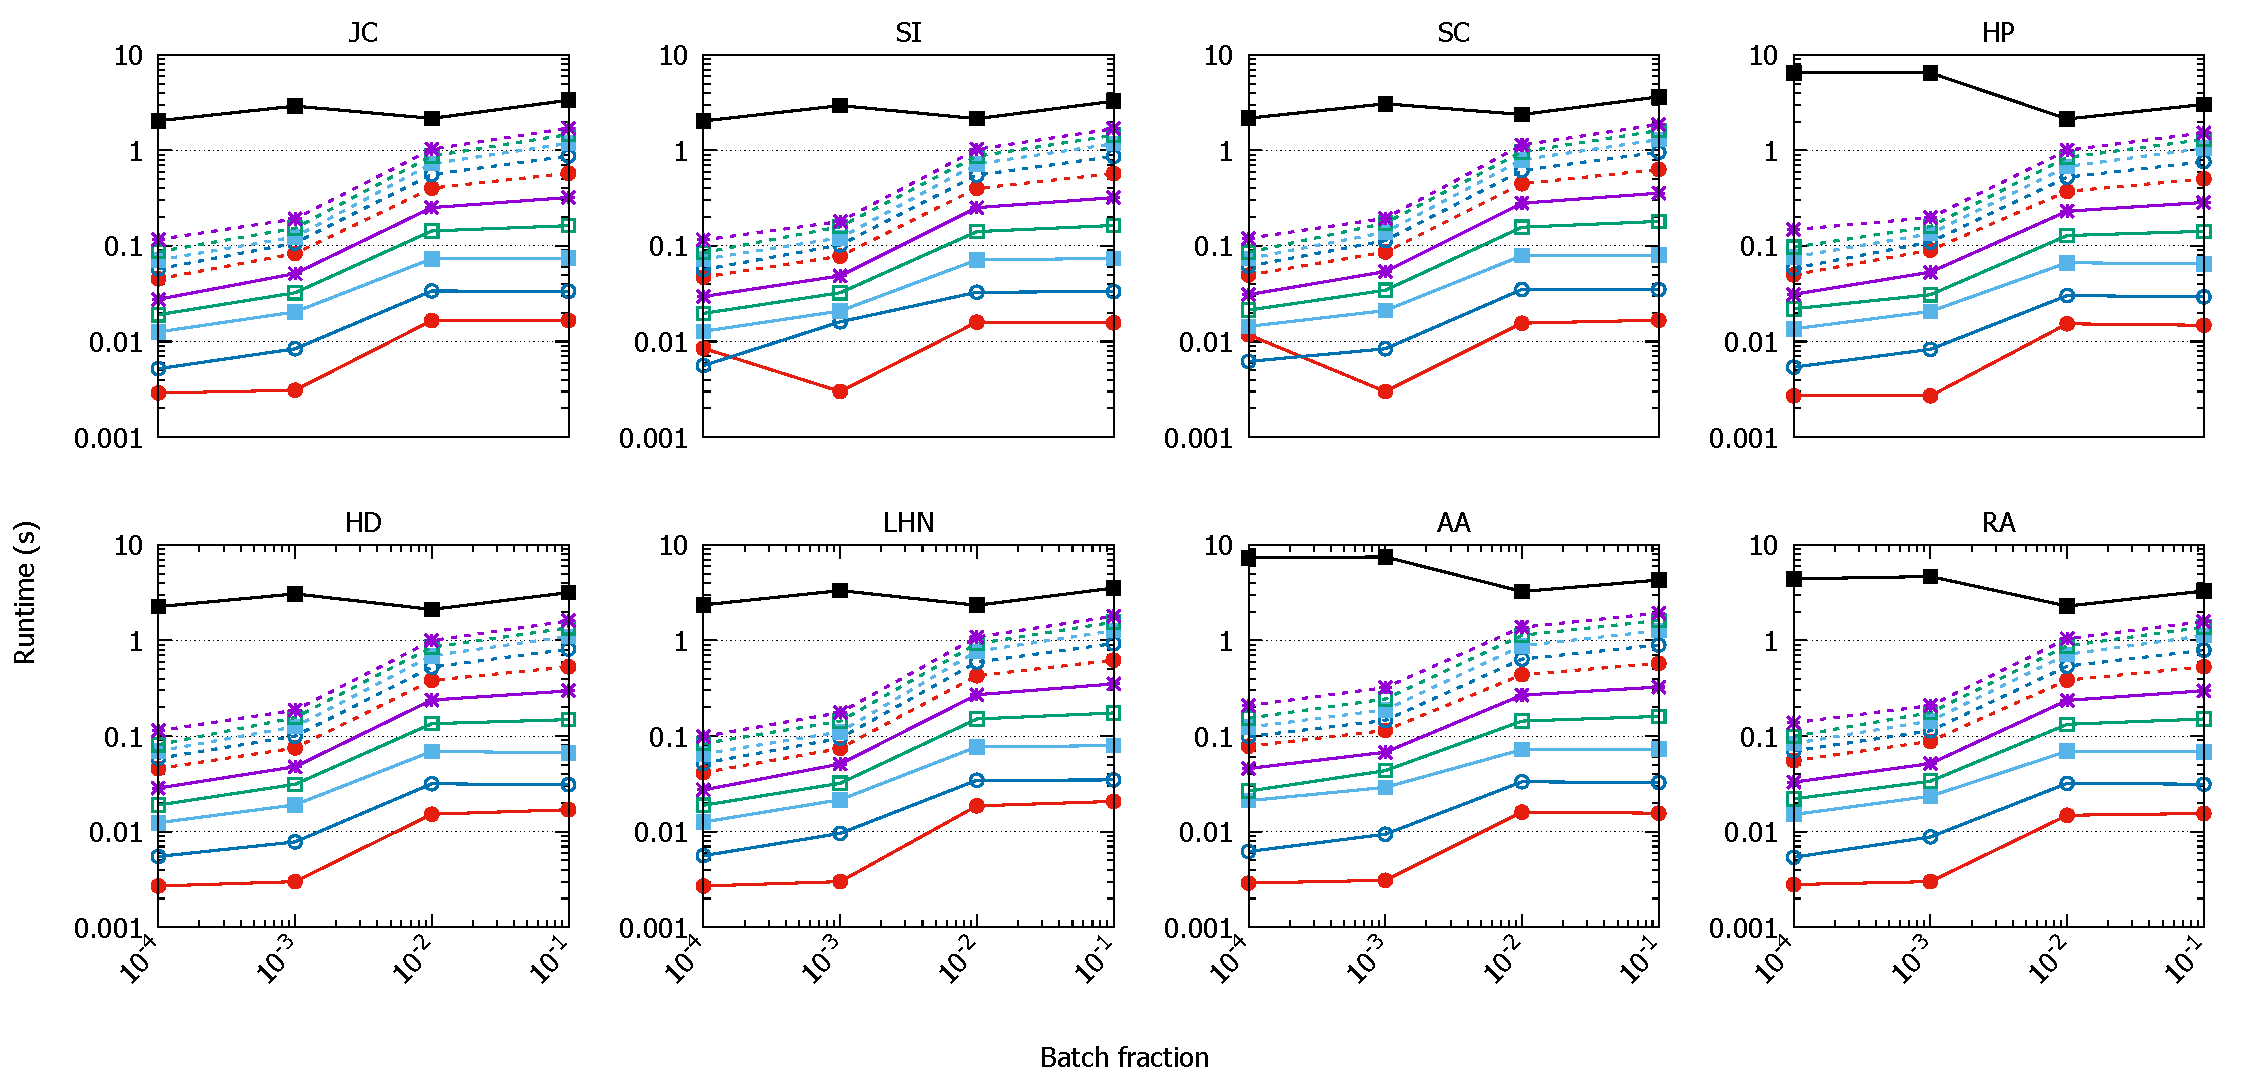
\includegraphics[width=0.98\linewidth]{out/adjust-mindegree-runtime.pdf}
  }
  \subfigure[F1 score of predicted links (logarithmic scale), of each link prediction method]{
    \label{fig:adjust-mindegree--precision}
    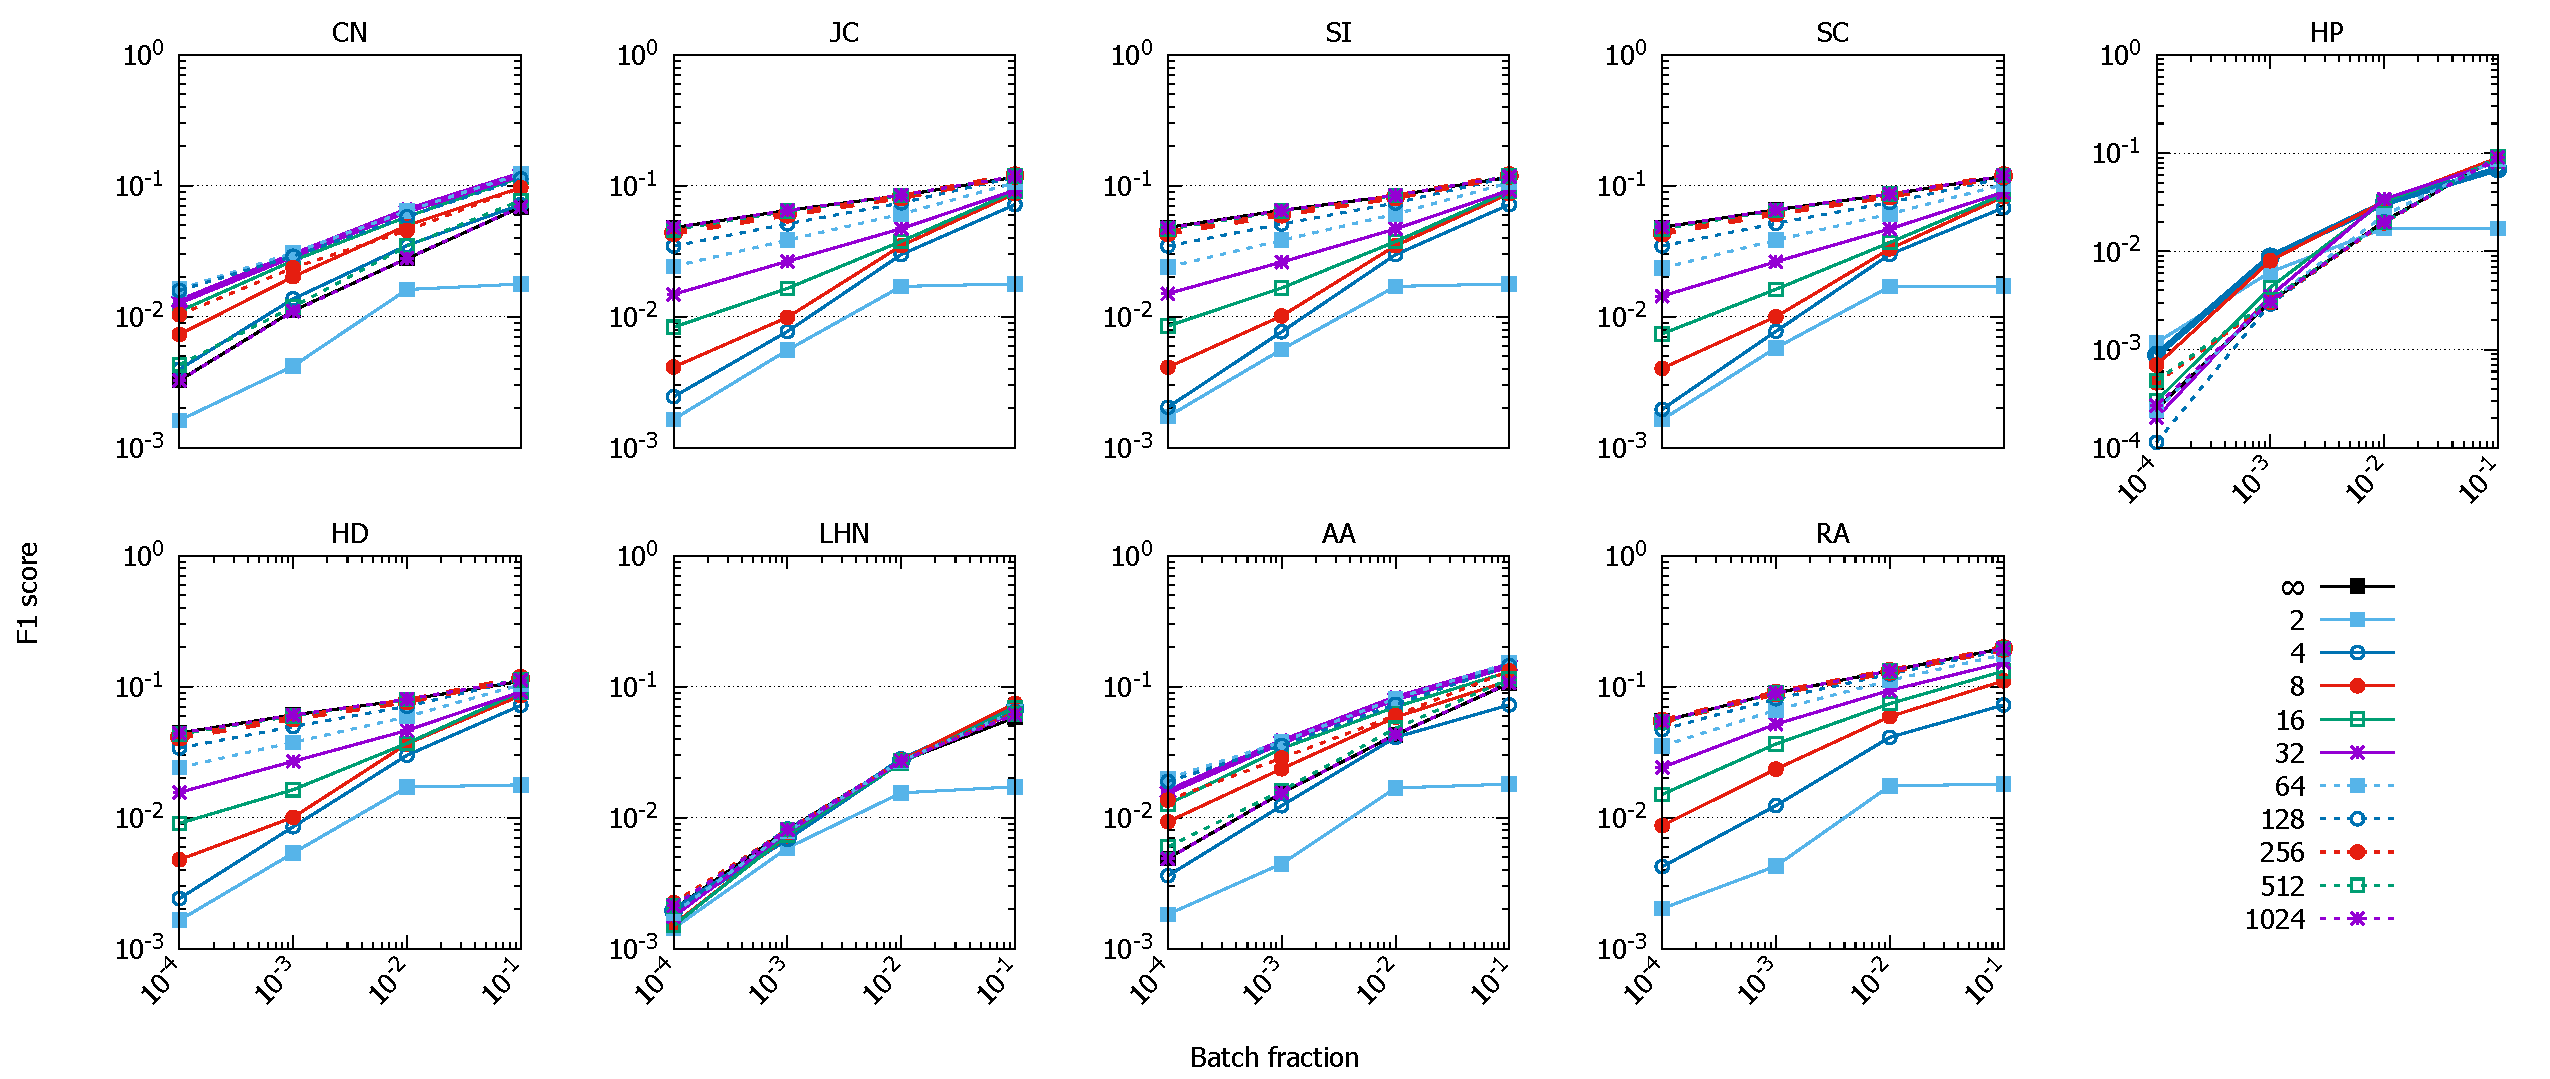
\includegraphics[width=0.98\linewidth]{out/adjust-mindegree-f1score.pdf}
  } \\[0ex]
  \caption{Impact of adjusting the \textit{MAX\_MEDIATOR\_DEGREE} from $2$ to $1024$ (in multiples of $2$), and to $\infty$, on the runtime (in seconds, log-scale), and precision of predicted links (in percentage, log scale), of each neighbor-based link prediction method, on batch sizes of $10^{-4}|E|$ to $0.1|E|$. The full form of each link prediction method is given in Section X.}
  \label{fig:adjust-mindegree}
\end{figure*}

\begin{algorithm}[hbtp]
\caption{Our Parallel \textit{Disregard Large Hubs (DLH)} approach.}
\label{alg:predict}
\begin{algorithmic}[1]
\Require{$G(V, E)$: Input graph}
\Require{$N_P$: Maximum number of edges to predict}
\Require{$S_{th}$: Threshold score above which to predict}
\Ensure{$a, b, c$: Current vertex, first-order, second-order neighbor}
\Ensure{$L_H$: Hub limit, i.e., large hub degree threshold}
\Ensure{$|\Gamma_b|$: Degree of first-order neighbor $b$}
\Ensure{$H_t$: Collision-free per-thread hashtable}
\Ensure{$P_t$: Per-thread prediction list}
\Ensure{$P_h$: Heap for merging per-thread prediction lists}
\Ensure{$P$: Global prediction list}

\Statex

\Function{predictLinksDLH}{$G, N_P, S_{th}$} \label{alg:predict--begin}
  \State $\rhd$ Scoring phase
  \State $P_t \gets \{\}$ \textbf{on each thread} \label{alg:predict--scoring-begin}
  \ForAll{$a \in V$ \textbf{in parallel}}
    \State $\rhd$ Scan second-order neighbors of $a$
    \State $H_t \gets \{\}$
    \ForAll{$b \in G.out(a)$}
      \State $\rhd$ Skip high degree first-order neighbors
      \If{$|\Gamma_b| \leq L_H$} $scanEdges(H_t, G, b)$
      \EndIf
    \EndFor
    \State $\rhd$ Avoid first-order neighbors
    \ForAll{$b \in G.out(a)$} $H_t[b] \gets 0$ \label{alg:predict--avoid-neighbors1}
    \EndFor
    \State $\rhd$ Get prediction scores and add to list
    \ForAll{$c \in H_t.keys()$}
      \State $score \gets computeScore(a, c, H_t[c])$
      \If{$score \leq S_{th}$} \textbf{continue}
      \EndIf
      \State $\rhd$ Add edge $(a, c)$ to prediction list
      \If{$|P_t| < N_P$}
        \State $P_t.push(\{a, c, score\})$
        \If{$|P_t| = N_P$} $P_t.makeMinHeapByScore()$
        \EndIf
      \ElsIf{$score \geq P_t[0].score$}
        \State $P_t.popHeap()$
        \State $P_t.pushHeap(\{a, c, score\})$
      \EndIf
    \EndFor
  \EndFor \label{alg:predict--scoring-end}
  \State $\rhd$ Merging phase \label{alg:predict--merging-begin}
  \State $P \gets \{\}$ \textbf{;} $P_h \gets \{\}$
  \State $sort(P_t)$ \textbf{on each thread}
  \ForAll{$t$ in threads}
    \If{$|P_t| \neq 0$} $P_h.push(\{t, P_t.back().score\})$
    \EndIf
  \EndFor
  \State $P_h.makeMaxHeapByScore()$ 
  \While{$|P_h| \neq 0$ \textbf{and} $|P| < N_P$} \label{alg:predict--merge-loop-begin}
    \State $t \gets P_h.popHeap().t$
    \State $P.push(P_t.back())$
    \State $P_t.pop()$
    \If{$|P_t| \neq 0$} $P_h.pushHeap(\{t, P_t.back().score\})$
    \EndIf
  \EndWhile \label{alg:predict--merging-end}
  \Return{$P$}
\EndFunction \label{alg:predict--end}

\Statex

\Function{scanEdges}{$H_t, G, a, b$} \label{alg:predict--scan-begin}
  \ForAll{$c \in G.out(b)$}
    \State $\rhd$ Skip reverse edges
    \If{$c \leq a$} \textbf{continue}
    \EndIf
    \If{$metric = AA$} $H_t[c] \gets H_t[c] + 1 / log(|\Gamma_b|)$
    \ElsIf{$metric = RA$} $H_t[c] \gets H_t[c] + 1 / |\Gamma_b|$
    \Else\ $H_t[c] \gets H_t[c] + 1$
    \EndIf
  \EndFor
\EndFunction \label{alg:predict--scan-end}
\end{algorithmic}
\end{algorithm}

